% !TeX root=../main.tex
\chapter{مروری بر مطالعات انجام شده}
%\thispagestyle{empty} 
\section{مقدمه}
در این فصل به مرور تعدادی از مقالات مربوط به استراتژی ذخیره‌سازی و سیاست جایگزینی محتوا در حافظه برای شبکه‌های اینترنت اشیا می‌پردازیم. در ادامه الگوریتم‌های استفاده شده در مقالات، معماری به کار رفته برای پیاده‌سازی و چالش‌های آن برای محیط  استفاده شده به طور اجمالی بیان می‌شوند. 

\section{مروری بر ادبیات موضوع}

\subsection{\lr{Deep Reinforcement Learning for Cooperative Content Caching in Vehicular Edge Computing and Networks}}
با توجه به ماهیت محیط و حرکت گره‌های مصرف کننده،‌در مقاله‌ی \cite{qiao2019deep} تعریف حالت با آنچه که پیشتر دیدیم تفاوت‌هایی دارد، در ضمن فضای اعمال مجاز نیز دیگر گسسته نخواهد بود که بتبع این مسئله پیچیدگی‌های بسیاری را به وجود می آورد. در ابتدا درباره‌ی فضای استیت‌ها و اکشن‌ها توضیحاتی داده می‌شود:

\paragraph{فضای استیت‌ها}
در ابتدای هر بازه‌ی زمانی، عامل هوشمند به اطلاعاتی درباره‌ی محتوای درخواستی توسط وسایل نقلیه\footnote{\lr{content requesting vehicles(CRV)}} دست پیدا می‌کند که این اطلاعات حالت عامل در این بازه‌ی زمانی را برای ما مشخص می‌کند و این مؤلفه‌ها عبارتند از:  
\begin{itemize}
	\item 
	نوع محتوای درخواست شده در بازه‌ی زمانی ذخیره‌سازی 
	\item 
	مهلت تحویل دیتای درخواستی در بازه‌ی زمانی ذخیره‌سازی کنونی
	\item
	سایز باقیمانده از دیتای درخواستی برای ارسال در بازه‌ی زمانی کنونی
	\item
	مؤلفه‌ی مربوط به منطقه‌ای که دیتای مربوط به محتوای درخواستی موجود بوده یا مؤلفه‌ی مربوط به موقعیتی که دیتای درخواستی ذخیره شده است.
	\item 
	میزان محبوبیت محتوای درخواستی در بازه‌ی زمانی فعلی
	\item 
	بیانگر عملیات ذخیره‌سازی\footnote{\lr{caching indicator}} که نشان می‌دهد در بازه‌ی زمانی ذخیره‌سازی فعلی، ذخیره‌ی دیتای درخواستی در کدام گره ذخیره‌سازی انجام شود.
\end{itemize}

\paragraph{فضای اکشن‌ها}
بعد از دریافت درخواست محتوا، رسانه‌ی همه‌پخشی ماهواره‌ای\footnote{\lr{Media Broadcast Satellite(MBS)}} محبوبیت محتوای درخواست شده را محاسبه می‌کند و از روی آن تصمیم می‌گیرد که‌ آیا لازم است دیتای مربوط به محتوای درخواستی ذخبره شود یا خیر و در صورتیکه پاسخ مثبت باشد،‌ گره مناسب برای ذخیره‌ی دیتا را مشخص می‌نماید. در هر بازه‌ی زمانی مربوط به واکشی پاسخ، مقادیر زمان‌بندی برای هریک از وسایل و نیز پهنای باند تخصیص یافته به هرکدام، توأماً برای کاهش هزینه‌ی دسترسی به محتوا با قید مهلت مربوط به ارسال پاسخ مورد استفاده قرار می‌گیرند. بنابراین فضای اکشن‌ها با مؤلفه‌هایی که در ادامه توصیف می‌شوند، مشخص می‌گردد.
\begin{itemize}
	\item 
	آیا محتوای درخواستی در بازه‌ی زمانی ذخیره‌سازی در حافظه وجود داشته است یا خیر. در صورتیکه جواب مثبت باشد، مقدار این مؤلفه 1 خواهد بود.  
	\item 
	نشانگر ارتباط\footnote{\lr{association indicator}} بین محتوای درخواستی و گره لبه، در واقع این مولفه مشخص می‌کند تا برای واکشی پاسخ باید به سراغ کدامیک از گره‌های لبه برویم.
	\item
	پهنای باندی که به ازای آن ارتباط بین گره لبه و وسیله‌ی درخواست دهنده برقرار می‌شود.
\end{itemize}
 
 در اینجا با توجه به پیوسته بودن فضای استیت‌ها و به طور ویژه اکشن‌ها به جای تخمین ارزش استیت ها یا ارزش استیت‌-اکشن‌ها (که به کمک شبکه یا شبکه‌ها‌ی عصبی صورت می‌پذیرد) ، به طور مستقیم سیاست بهینه را با استفاده از الگوریتم \lr{Deep Deterministic Policy Gradient}(\ref{fig:DDPG}) تخمین می‌زنیم.
 \begin{figure}[ht]
 	\centerline{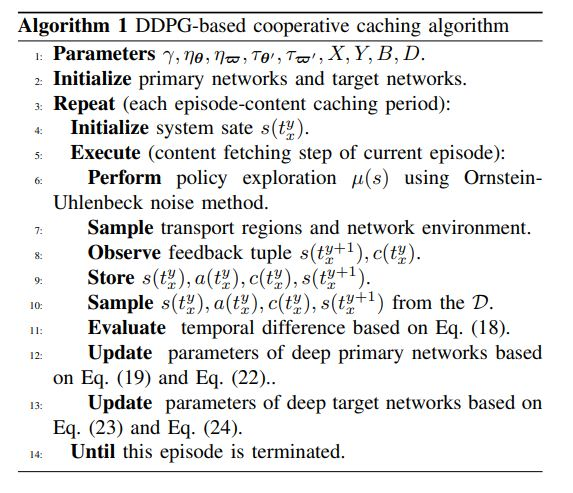
\includegraphics[width=11cm]{DDPG}}
 	\caption{الگوریتم \lr{Deep Deterministic Policy Gradient}}
 	\label{fig:DDPG}
 \end{figure}

الگوریتم پیشنهادی مقاله در زمره‌ی یادگیری بدون مدل\footnote{\lr{Model-free Learning}} به‌ شمار می‌رود که براساس تعداد بسیاری از تجربیات و تعاملات با محیط، تخمین سیاست صورت می‌پذیرد. برای بیان چرایی و مزیت این الگوریتم نسبت به سایر الگوریتم‌های مشابه، در ادامه توضیحاتی درباره‌ی سه مدل مختلف یادگیری بدون مدل ارائه می‌گردد. 

\begin{itemize}
	\item \textbf{مدل مبتنی بر ارزش\footnote{\lr{value-based approach}} یا مدل نقاد\footnote{\lr{critic model}}}\\
	در این روش، سیاست بهینه براساس مقادیر مربوط به تخمین ارزش استیت-اکشن‌ها \lr{$Q(s, a)$} به دست می‌آید. 
	\item \textbf{مدل مبتنی بر سیاست\footnote{\lr{policy-based approach}} یا مدل عملگر\footnote{\lr{actor model}}}\\
	این روش می‌تواند سیاست مبتنی بر احتمالات (احتمال قرار گرفتن در یک استیت مشخص با توجه به غیرایستان بودن محیط) \lr{$\pi_{\overline{\omega}}(s|a)$} را یاد بگیرد.
	
	\item \textbf{روش عملگر-نقاد\footnote{\lr{actor-critic}}}\\
	این روش ترکیبی از دو روش قبلی می‌باشد که در این مقاله به کمک الگوریتم \lr{policy gradient} در عملگر، سیاست بهینه تخمین زده می‌شود و براساس فیدبکی که نقاد برای ارزش استیت-اکشن‌ها تولید می‌کند، سیاست مذکور اصلاح می گردد. درواقع این دست از الگوریتم‌ها برای هر دو فضای اکشن‌های پیوسته و گسسته مناسب می‌باشند که نمونه‌ی گسسته‌ی آن را در ادامه می‌بینیم. البته همگرایی و کارآمدی الگوریتم‌های عملگر-نقاد به تعداد نمونه‌ها و تعاملات با محیط وابسته است.
	
\end{itemize}

\begin{figure}[ht]
	\centerline{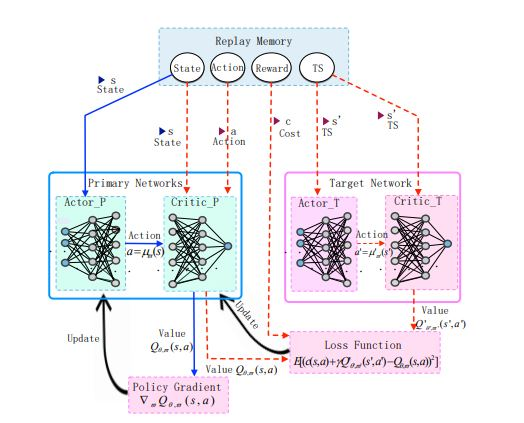
\includegraphics[width=10cm]{PG}}
	\caption{دیاگرام \lr{Deep Deterministic Policy Gradient}}
	\label{fig:PG}
\end{figure}

 همانطوری که در شکل \ref{fig:PG} مشاهده می‌شود، این مقاله از شبکه‌های عصبی عمیق برای تخمین دقیق تابع قطعیت سیاست\lr{$\mu(s)$} و ارزش استیت-اکشن‌هاlr{$Q(s, a)$} استفاده می‌کند. همانطوری که می‌بینید فریمورک به کار رفته از سه ماژول اصلی تشکیل می‌شود: شبکه‌های مقدماتی\footnote{\lr{primary networks}}، هدف\footnote{\lr{target networks}} ( که در هریک شبکه‌های عمیق عملگر\footnote{\lr{deep actor-network}} و نقاد\footnote{\lr{deep critic-network}} نقش اصلی را ایفا می‌کنند) و حافظه‌ی بازپخشی\footnote{\lr{replay memory}}.

\subsection{\lr{Caching Transient Content for IoT Sensing: Multi-Agent Soft Actor-Critic}}
در مقاله‌ی \cite{wu2021caching} برای اولین بار راه حلی برای مسئله‌ی به روز رسانی حافظه‌ی کش برای یک محیط چندعامله و متشکل از چندین گره لبه ارائه شده و این مسئله به صورت یک فرآیند تصمیم‌گیری مارکوف مشارکتی بین چندعامل براساس کاهش مقدار تابع وزنداری از طول عمر آیتم هر محتوا، هزینه‌ی به روزرسانی حافظه‌ی ذخیره‌سازی، بارترافیکی شبکه و کاهش مصرف انرژی در واکشی پاسخ مطرح گردیده است. 

در اینجا یک نسخه از الگوریتم چندعامله‌ی \lr{Soft Actor-Critic} با فضای اعمال گسسته ایجاد شده است که تعداد عامل‌های الگوریتم خروجی به طور خطی با تعداد گره‌های لبه و حسگرهای شبکه‌های اینترنت اشیا قابل افزایش است. برای رسیدن به این هدف، در این مقاله از یک \lr{Gumble-SoftMax-sampler} برای نمونه‌برداری از محیط استفاده شده است که پارامترهای مربوط به آن را برای رسیدن به فضای اعمال دیفرانسیل‌پذیر تنظیم می‌نماید. در آخر نیز برای برقرای توازن میان اکتشاف و بهره‌وری (که مسئله‌ی مشترک میان تمامی الگوریتم‌های یادگیری تقویتی می‌باشد) از یک تنظیم‌ساز آنتروپی\footnote{\lr{Entropy Regularization}} برای جلوگیری از همگرایی زودهنگام استفاده می‌شود.

برای کاهش سربار ارتباط میان گره‌های لبه و لایه‌ی ابری، هریک از الگوریتم‌های \lr{Soft Actor-Critic} و \lr{Deep Q-Network} در دو حالت روش کنترلی متمرکز و غیرمتمرکز پیاده‌سازی و مقایسه شده‌اند. در سیاست کنترلی غیرمتمرکز\ref{fig:decentralized}، هرکدام از سرورهای گره‌های لبه به عنوان یک عامل مستقل، براساس مشاهدات خود تصمیماتی را برای ذخیره‌کردن، جایگزینی محتوا و ... اتخاذ می‌نماید اما در روش کنترلی متمرکز\ref{fig:centralized} از یک پردازنده‌ی ابری\footnote{\lr{Cloud Processor}} برای بهبود پاداش‌های دریافتی سیستم و بالا بردن هماهنگی با سایر گره‌های لبه استفاده می‌شود.

\begin{figure}[ht]
	\centering 
	\subfloat[روش کنترلی متمرکز]{ \label{fig:centralized}
		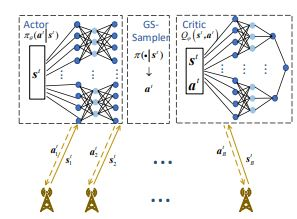
\includegraphics[width=0.4\textwidth]{centralized}}
	\hspace{10mm}
	\subfloat[روش کنترلی غیرمتمرکز]{ \label{fig:decentralized}
		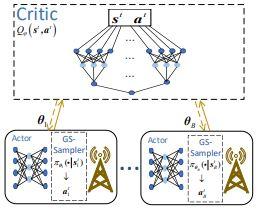
\includegraphics[width=0.4\textwidth]{decntralized}}%
	\caption{دیاگرام الگوریتم \lr{SAC} به کاررفته}
	\label{fig:centralizedvsdec} %% label for entire figure
\end{figure}
\pagebreak

همانطوری که در شکل \ref{fig:centralizedvsdec} دیده می‌شود، در الگوریتم متمرکز، پردازنده‌ی ابری نقش یک عامل متمرکز را ایفا می‌کند و سیاست متمرکز برای تمامی گره‌های لبه را یاد می‌گیرد. متناسباً هریک از گره‌های لبه ابتدا مشاهدات خود را در هر واحد زمانی برای پردازنده‌ی ابری می‌فرستند و سپس پس از آنکه پردازنده‌ی ابری مشاهدات محلی آنها را جمع‌آوری کرد، عملکرد بهینه برای هریک از گره‌های لبه را ارسال می‌نماید. 

در آخر نیز، عملکرد الگوریتم \lr{SAC} در حالت متمرکز و غیر متمرکز با روش‌های عملگر-نقاد معمول و روش \lr{DQN} مقایسه شده است. به طور کلی، متوسط پاداش دریافتی برای \lr{Decentralized SAC} نسبت به \lr{Centralized SAC} بیشتر بوده و مقدار به دست آمده حاصل از الگوریتم \lr{Centralized SAC} از الگوریتم عملگر-نقاد معمول بیشتر بوده و برای الگوریتم عملگر-نقاد معمول نسبت به \lr{DQN} بیشتر است و البته باید به این نکته اشاره کرد که متوسط پاداش به دست آمده برای الگوریتم \lr{DQN} نسبت به سایر الگوریتمها نویزی‌تر نیز می‌باشد. 


%\begin{figure}[ht]
%	\centerline{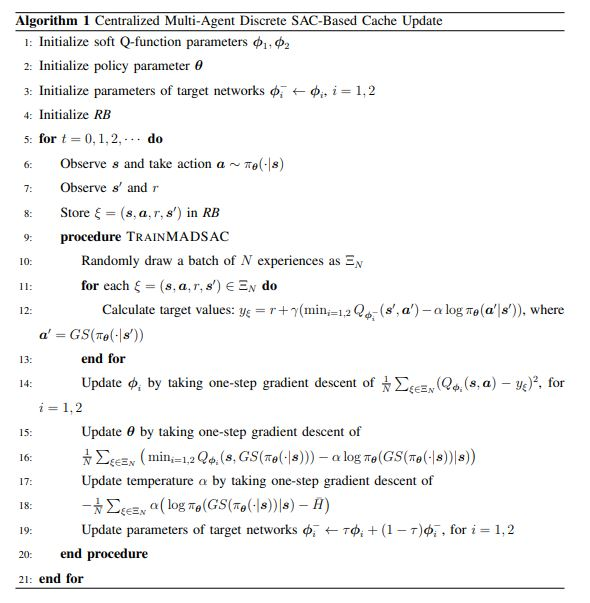
\includegraphics[width=8cm]{centralizedSAC}}
%	\caption{الگوریتم \lr{Centralized Soft Actor-Critic}}
%	\label{fig:cSACAlgo}
%\end{figure}

%\begin{figure}[ht]
%	\centerline{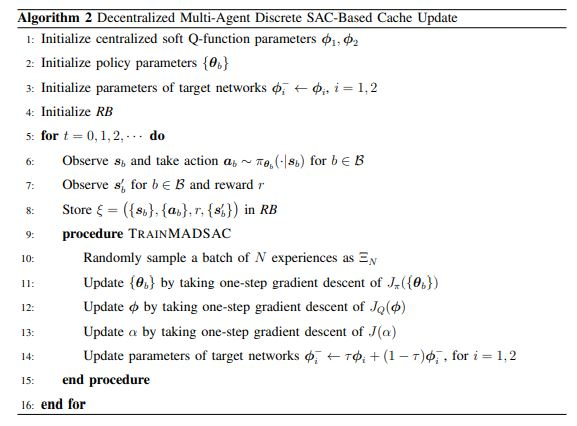
\includegraphics[width=8cm]{decentralizedSAC}}
%	\caption{الگوریتم \lr{Decentralized Soft Actor-Critic}}
%	\label{fig:dSACAlgo}
%\end{figure}

\subsection{\lr{A Deep Reinforcement Learning-Based Caching Strategy for IoT Networks with Transient Data}}

مقاله‌ی \cite{wu2022deep} از وجود لایه‌های مختلف در معماری شبکه‌های اینترنت اشیا بهره می‌برد و مدلی متشکل از دو لایه با یک گره پدر\footnote{\lr{parent node}} در لایه‌ی بالایی و چندین گره برگ\footnote{\lr{leaf}} یا لبه در لایه‌ی پایین‌تر شبکه در نظر می‌گیرد و تمامی این گره‌ها از قابلیت ذخیره‌سازی برخوردارند. شکل \ref{fig:parent-leaf} معماری در نظر گرفته شده در این مقاله را نشان می‌دهد.

\begin{figure}[ht]
	\centerline{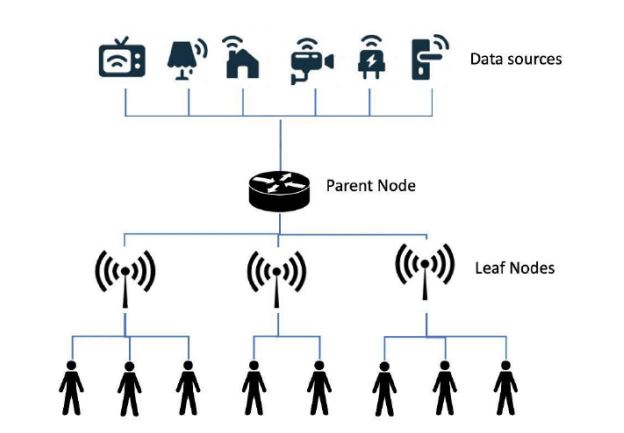
\includegraphics[width=10cm]{parent-leaf}}
	\caption{نمایی از معماری ریشه-برگ}
	\label{fig:parent-leaf}
\end{figure}

بنابراین می‌توان گفت که شبکه‌های اینترنت اشیا موجودیت‌های مختلفی از جمله افزاره‌های شبکه‌های اینترنت اشیا، گره ریشه، گره‌های برگ یا لبه و کاربران را شامل می‌شوند. 

\begin{itemize}
	\item \textbf{افزاره‌های شبکه‌های اینترنت اشیا}\\
	این افزاره‌ها در دنیای فیزیکی تعبیه می‌شوند و از آنها انتظار می‌رود تا پارامتری در محیط را اندازه‌گیری کرده و گزارش دهند یا بخشی از محیط را کنترل نمایند. گاهی نیز ممکنست اعتبار داده‌ی گزارش شده توسط آنها به حدی کم باشد که عملاً فایل تولید شده قابل ذخیره‌سازی نباشد.
	\item \textbf{گره ریشه}\\
	این نوع از گره‌ها لایه‌های درونی شبکه را شکل می‌دهند و مانند درگاهی که از یک طرف تمامی افزازه‌های شبکه‌ی اینترنت اشیا به تمامی گره‌های لبه یا برگ از طرف دیگر متصل می‌کند، عمل می‌نماید. درواقع این گره درخواست را از طرف گره‌های لبه دریافت می‌کند و پاسخ را از افزاره‌های مربوطه واکشی کرده و سپس برای گره‌های لبه می‌فرستد.
	\item \textbf{گره برگ}\\
	این دسته از گره‌ها نزدیکترین درگاه به کاربران هستند و میزان پوشش آنها به صورت منطقه‌ای و در حد تعدادی از کاربران می‌باشد، این گره‌ها به گره ریشه متصل هستند. 
	\item \textbf{کاربران}\\
	درواقع منظور از کاربران می‌تواند اپلیکیشن‌هایی برای پایش دیتای تولیدشده توسط حسگرها باشد. در این مقاله فرض شده است که حرکت کاربران محدود بوده و اتصال بین کاربر و گره برگ پایدار است در واقع این بدین معنیست که کاربر از دامنه‌ی پوشش گره برگ قبل از رسیدن پاسخ خارج نمی‌شود. 
\end{itemize}

این مقاله برای مشخص کردن رتبه‌بندی فابل‌ها به لحاظ محبوبیت در استراتژی ذخیره‌سازی و جایگزینی محتوا از الگوریتم \lr{Proximal Policy Optimization} (\ref{fig:ppo}) به سبک عملگر-نقاد در دو حالت متمرکز و غیرمتمرکز استفاده می‌کند. در حالت متمرکز هریک از گره‌های برگ تصمیمات مربوط به ذخیره‌سازی یا جایگزینی محتوا در حافظه را می‌گیرد اما در حالت غیرمتمرکز گره ریشه بر روی تصمیمات ذخیره‌سازی اثر می‌گذارد و محتویات 
ذخیره‌سازی در هریک از گره‌های برگ را مشخص می‌کند و محتویات مشترک میان آنها در گره ریشه ذخیره می‌گردد.

\begin{figure}[ht]
	\centerline{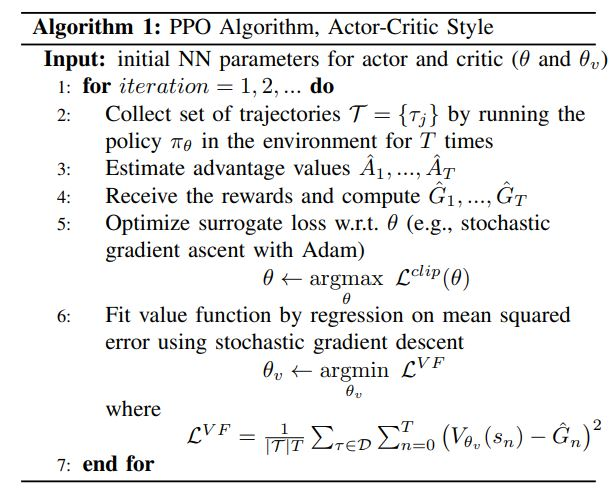
\includegraphics[width=11cm]{PPO}}
	\caption{الگوریتم \lr{Proximal Policy Optimization}}
	\label{fig:ppo}
\end{figure}

همانطوری که در شکل \ref{fig:ppo} می‌بینید در اینجا نیز از یک سیاست پارامترایز شده \lr{$\pi_{\theta}(a|s)$} برای تخمین محبوبیت فایل‌ها در محیط غیرایستان استفاده می‌شود که برای محیط‌های چندعامله نیز قابل پیاده‌سازی است و به این دلیل این الگوریتم نیز در گروه الگوریتم‌های \lr{policy gradient} قرار می‌گیرد. در اینجا نیز دو شبکه‌ی عصبی عملگر برای تخمین سیاست و نقاد برای تخمین ارزش استیت‌ها \lr{$V^{\pi_{\theta}}(s; \theta_{\nu})$} به کار رفته‌اند. علاوه بر حل مسئله‌ی بهینه‌سازی برای یافتن سیاست بهینه، یکی از اهداف الگوریتم بهینه‌سازی تابع \lr{clipped Surrogate} که از \lr{stochastic gradient ascent} استفاده می‌کند، می‌باشد. در واقع از این تابع برای آپدیت پارامتر سیاست بهینه با پارامتر \lr{$\theta$} توسط شبکه‌ی عملگر براساس فیدبک نقاد طبق مشاهدات در تعامل با محیط استفاده می‌شود. تابع هدف \lr{clipped Surrogate} به صورت 
\begin{equation}\label{eq:20}
	\mathcal{L}^{clip}(\theta) = E_{\pi}[\min(b_n(\theta)A_n, clip(b_n(\theta), 1 - \epsilon, 1 + \epsilon)A_n)]
\end{equation}  
\begin{equation}\label{eq:21}
	b_n(\theta) = \frac{\pi_{\theta}(a_n|s_n)}{\pi_{\theta_{old}}(a_n|s_n)}
\end{equation}  
تعریف می‌شود.

درواقع تابع \lr{$clip$} یک نسبت احتمالاتی \lr{$b_n(\theta)$} را که مطابق با رابطه‌ی \ref{eq:21} تعریف می‌شود، از ورودی می‌گیرد که اگر مقدار آن از \lr{$1-\epsilon$} کمتر و یا از \lr{$1+\epsilon$} بیشتر نباشد، همان را به عنوان خروجی برمی‌گرداند و در غیر اینصورت یکی از این مقادیر را جایگزین می‌نماید. همانطوری که می‌دانید \lr{$\theta_{old}$} مقدار پیشین این پارامتر قبل از آپدیت می‌باشد و مقدار \lr{$A_n$} به صورت
\begin{equation}\label{eq:20}
	A_n = r_n +‌\gamma V^{\pi_{\theta}}(s_{n+1}) - V^{\pi_{\theta}}(s)
\end{equation}  
تعریف می‌شود و مقداار \lr{$\theta$} به صورت
\begin{equation}\label{eq:20}
	\theta \leftarrow \arg\max \mathcal{L}^{clip}(\theta)
\end{equation}
آپدیت می‌شود.

در نهایت نیز همانطوری که مورد انتظار است، متوسط مجموع پاداش‌های دریافتی در حالت غیرمتمرکز (در حالیکه فرمان ذخیره یا جایگزینی محتوا از سوی گره ریشه به گره های برگ صادر می‌شود) نسبت به حالت متمرکز به مقدار بیشتری همگرا می‌شود و با به کار گرفتن روش کنترلی غیرمتمرکز در محیط ذکر شده در مقاله، مقدار تأخیر و ترافیک در شبکه متوازن‌تر می‌شود.
\pagebreak
در شکل \ref{fig:ppod} دیاگرام مربوط به الگوریتم \lr{Proximal Policy Optimization} در مقاله‌ی \cite{wu2022deep} آورده شده است.

\begin{figure}[ht]
	\centerline{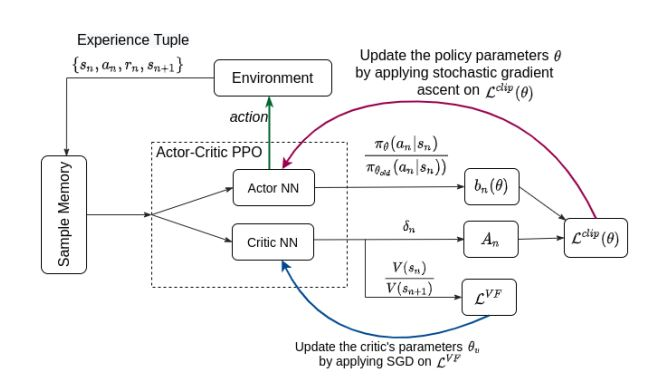
\includegraphics[width=14cm]{PPO-diagram}}
	\caption{دیاگرام \lr{Proximal Policy Optimization}}
	\label{fig:ppod}
\end{figure}

\newpage
\subsection{\lr{HFDRL: An Intelligent Dynamic Cooperate Cashing Method Based on Hierarchical Federated Deep Reinforcement Learning in Edge-Enabled IoT}}

در الگوریتم یادگیری تقویتی عمیق فدراسیونی سلسله مراتبی\footnote{\lr{Hierarchical Federated Deep Reinforcement Learning}} پیشنهادی مقاله‌ی \cite{majidi2021hfdrl}، ابتدا به صورت سلسله مراتبی گره‌های لبه با استفاده از الگوریتم \lr{Fuzzy C-Means} طبقه‌بندی می‌شوند. اساس طبقه‌بندی پارامترهایی مانند موقعیت جغرافیایی، ویژگی‌های مربوط به کاربران (از قبیل سن، جنسیت و ...) و خصوصیات درخواست‌های ارسالی (از قبیل نوع،‌ دیتاسنتر مربوطه و ...)، می‌باشد که ماهیت غیرایستان بودن محیط نیز در خوشه‌بندی در نظز گرفته شدا است زیرا در طول زمان الگوی درخواست‌های ارسالی کاربران تغییر می‌کند. همانطوری که در شکل \ref{fig:cluster-levels} دیده می‌شود، خوشه‌های در طبقه‌بندی اول با کمترین میزان تأخیر می‌توانند ارتباط را برقرار کنند و بیشترین مبادله‌ی محتویات را داشته باشند. در سطح بعدی هرکدام از خوشه‌ها به منزله‌ی یک گره تلقی می‌گردند و خوشه‌بندی در لایه‌ی بعدی نیز عیناً طبق پارامترهای مورد استفاده در خوشه‌بندی لایه‌ی قبلی، انجام می‌پذیرد. در صورت نیاز به لایه‌های بیشتر، خوشه‌بندی در آنها به همین منوال صورت می‌گیرد. 

\begin{figure}[ht]
	\centerline{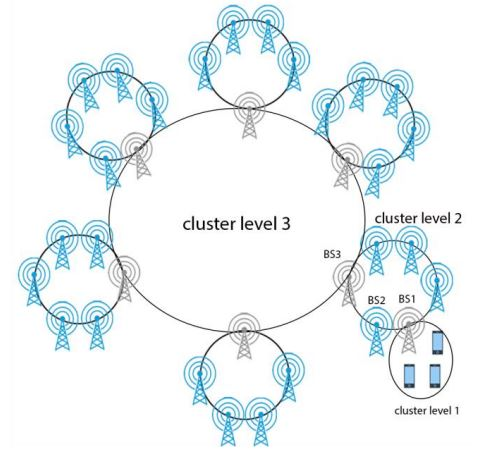
\includegraphics[width=10cm]{cluster-levels}}
	\caption{خوشه‌بندی سه‌لایه‌ای از ایستگاه‌های پایه}
	\label{fig:cluster-levels}
\end{figure}

در یادگیری تقویتی عمیق سلسله‌مراتبی و فدراسیونی هر کدام از گره‌های لبه در شبکه تابع ارزش استیت-اکشن‌ها را به کمک یک شبکه‌ی یادگیری تقویتی عمیق تخمین می‌زند و مقدار محبوبیت فایل‌ها زا نیز پیش‌بینی می‌کند و براساس آن دیتا را ذخیره کرده و یا آن را از حافظه حذف می‌نماید.  

پس از خوشه‌بندی هریک از گره‌های لبه،‌ هرگاه که درخواستی به ایستگاه پایه ارسال می‌شود ابتدا لازم است تا مشخص شود که آیا محتوای درخواست شده قبلاً ذخیره شده است یا خیر که در صورت مثبت بودن پاسخ باید ایستگا‌هی که دیتا در آن ذخیره شده مشخص شود. بدین منظور یک سرگروه از هر خوشه انتخاب می‌شود که شناسه‌ی محتوا و ایستگاه پایه‌ای که محتوا را ذخیره کرده، ثبت می‌نماید. اگر در هر بازه‌ی زمانی سرگروه خوشه تغییر کند، در هرتغییر سابقه‌ی قبلی خوشه(به لحاظ محتوای ذخیره شده و ایستگاه پایه مربوط به آن) به سرگروه جدید ارسال می‌شود و در صورتیکه محتوایی ازحافظه حذف یا بدان اضافه شود یک پیام به گره سرگروه ارسال می‌شود و جدول آن به روزرسانی می‌گردد. مکانیزم استفاده شده در مقاله را در شکل \ref{fig:hfdrl} مشاهده می‌کنید.

\begin{figure}[ht]
	\centerline{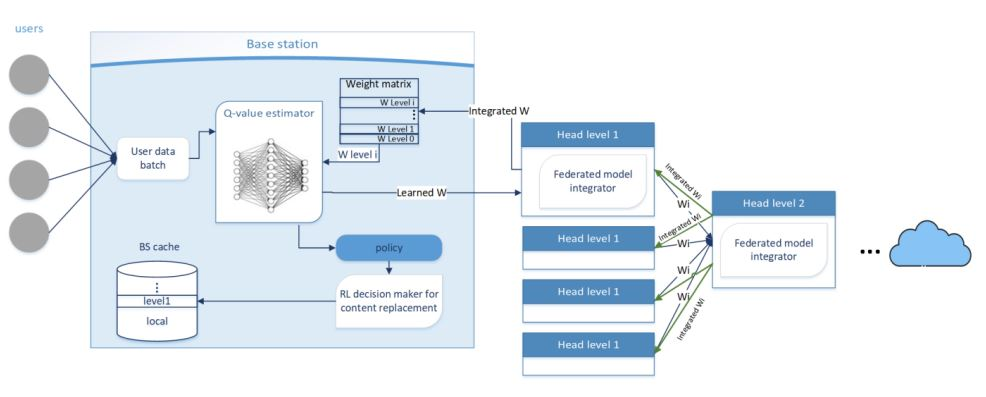
\includegraphics[width=15cm]{HFDRL}}
	\caption{مکانیزم تجمع مدل‌ها در معماری سلسله مراتبی فدراسیونی یادگیری تقویتی عمیق}
	\label{fig:hfdrl}
\end{figure}

 لازم به ذکر است که برای تعیین سرگروه، پارامترهایی چون زمان صرف شده برای دریافت محتوا با شناسه‌ی مشخص از دیتاسنتر تا گره مذکور، تعداد بارهایی که محتوا با شناسه‌ی مشخص از گره مذکور در خواست شده است و میزان حافظه‌ی لازم برای ذخیره‌ی محتوا، در نظر گرفته می‌شوند.
 
 پس از خوشه‌بندی گره‌ها در آغاز بازه‌ی زمانی،‌ هرگاه که ایستگاه پایه درخواستی را دریافت نماید، مراحل زیر را مطابق با شکل \ref{fig:fdrl} برای پاسخگویی دنبال می‌کند:
 \begin{enumerate}
 	\item 
 	در صورتیکه دیتا در حافظه‌ی محلی موجود باشد، به تعداد بارهای موفقیت آمیز در یافتن پاسخ از حافظه اضافه شده و در آخر نیز دیتا برای کاربر فراهم می‌گردد.
 	\item 
 	در صورتیکه محتوا در حافظه‌ی محلی موجود نباشد اما گره دیگری از خوشه آن را ذخیره کرده باشد، به تعداد بارهای موفقیت آمیز در یافتن پاسخ از حافظه اضافه شده و توسط ایستگاه پایه‌ی همگروه با آن دیتا برای کاربر ارسال می‌شود.
 	\item 
 	در صورتیکه محتوا در حافظه‌ی محلی و گره دیگری از خوشه موجود نباشد، درخواست به سطوح بالاتر رفته و در صورت موجود بودن به تعداد بارهای موفقیت آمیز در یافتن پاسخ از حافظه اضافه شده و توسط ایستگاه پایه‌ی مربوطه دیتا برای کاربر ارسال می‌شود.
 	\item 
 	در صورتیکه دیتا در حافظه‌ی محلی،‌ گره‌های خوشه و یا سطوح بالاتر وجود نداشته باشد، از دیتاسنتر مقدار مربوط به آن واکشی می‌شود. حال براساس میزان محاسبه شده برای محبوبیت محتوا دیتا در عمومی‌ترین لایه که حداقل میزان محبوبیت مربوط به آن را تأمین می‌نماید، ذخیره می‌گردد. 
 \end{enumerate}

\begin{figure}[ht]
	\centerline{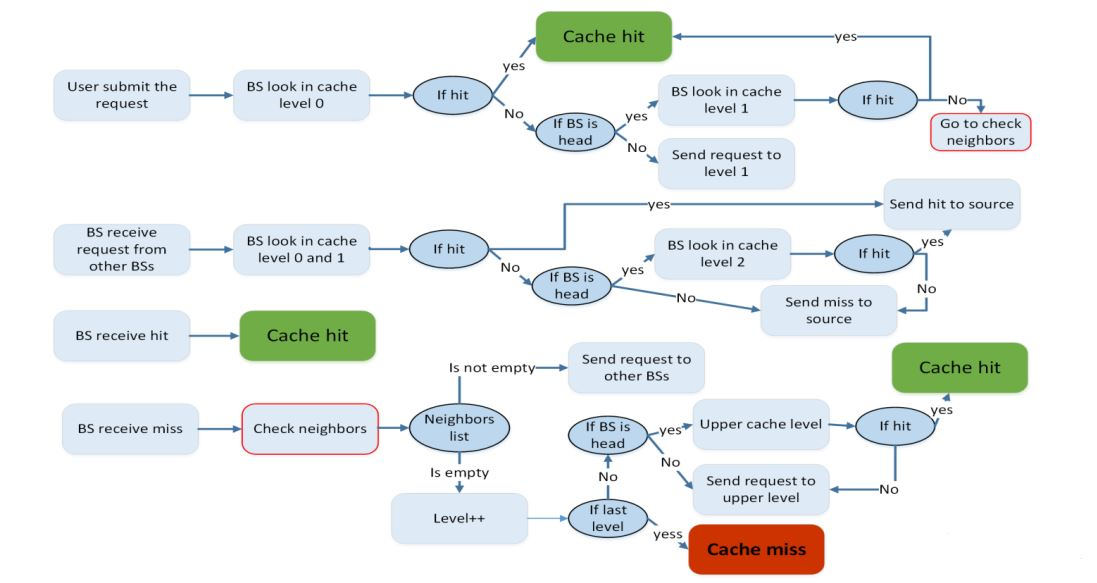
\includegraphics[width=15cm]{FDRL}}
	\caption{دیاگرام جریان داده برای پاسخ به درخواست‌های کاربران در مدل سلسله مراتبی و مشارکتی}
	\label{fig:fdrl}
\end{figure}

در آخر نیز دیده می شود که با خوشه‌بندی گره‌های لبه میزان موفقیت در ارسال پاسخ با ذخیره‌سازی افزایش می‌یابد. در این مقاله، لایه‌بندی‌ها نهایتاً تا سه لایه انجام می‌شود و کارآمدی استراتژی به کار رفته برای طبقه‌بندی سه لایه از طبقه‌بندی دولایه و برای طبقه‌بندی دو لایه نسبت به حالت تک لایه بیشتر می‌باشد.


